% REMEMBER TO SET LANGUAGE!
\documentclass[a4paper,10pt,english]{book}
\usepackage[utf8]{inputenc}
\usepackage{cite}
\usepackage{braket}
\usepackage{enumitem}
\usepackage{upgreek}
\usepackage{multicol}
\usepackage{mhchem}

% Standard stuff
\usepackage{amsmath,amsthm, amssymb,graphicx,varioref,verbatim,amsfonts,geometry,esint,url,color}
% colors in text
\usepackage[usenames,dvipsnames,svgnames,table]{xcolor}
% Hyper refs
\usepackage[colorlinks]{hyperref}
\usepackage{float}
\usepackage{wrapfig}
\usepackage{circuitikz}

\usepackage{tikz}
\usepackage[framemethod=tikz]{mdframed}
\usepackage{tikz-3dplot}
\usetikzlibrary{matrix,calc}

\usepackage{bm}

\usepackage[export]{adjustbox}

\usepackage{subfig}
\usepackage{algpseudocode}
\usepackage{algorithm}
\usepackage[makeroom]{cancel}

\usepackage{tcolorbox}
\tcbuselibrary{most}

%%%% PREVENT EXTRA WHITESPACE IN SECTION TITLES
\usepackage{sectsty}
\sectionfont{\raggedright}
%%%%

%%%%%FOR THE enumitem PACKAGE
\setlist[enumerate]{label*=\arabic*.}
%%%%%

%%%%EXAMPLE ENVIRONMENT

\newtcolorbox
[auto counter,number within=section]{pabox}[2][]{
%
enhanced,colback=black!5!white, colframe=black, fuzzy shadow={0mm}{-4pt}{-0.5pt}{0.4mm}{black!60!white},
title=Example 
\thetcbcounter
: #2,#1}

\newcommand{\example}[2]{
\begin{pabox}[label={myautocounter}]{#1}
#2
\end{pabox}
}
%%%%%%%%%%%%%%%%%%%%%%

%%%% BOX EQUATION ENVIRONMENT

\newenvironment{boxequation}{
\begin{tcolorbox}[ams equation, enhanced, colback=black!50!green!10!white, colframe=black, fuzzy shadow={0mm}{-4pt}{-0.5pt}{0.4mm}{black!60!white}]}
{\end{tcolorbox}}
%%%%%%%%%%%%%%%%%%%%%%%%%%%%%

%%%% BOX QUOTE ENVIRONMENT

\newenvironment{boxquote}{
\begin{tcolorbox}[enhanced, colback=black!50!green!10!white, colframe=black, fuzzy shadow={0mm}{-4pt}{-0.5pt}{0.4mm}{black!60!white}]
\begin{center}}
{\end{center}\end{tcolorbox}}

%%%%%%%%%%%%%%%%%%%%%%%%%%

% Document formatting
\setlength{\parindent}{0mm}
\setlength{\parskip}{1.5mm}


%Color scheme for listings
\usepackage{textcomp}
\definecolor{listinggray}{gray}{0.9}
\definecolor{lbcolor}{rgb}{0.9,0.9,0.9}

%Custom Math Operators
\DeclareMathOperator{\col}{col}
\newcommand{\colx}{\col x}

\DeclareMathOperator{\row}{row}
\newcommand{\rowx}{\row x}

\DeclareMathOperator{\nul}{nul}
\newcommand{\nulx}{\nul x}

\DeclareMathOperator{\rank}{rank}
\newcommand{\rankx}{\rank x}

\DeclareMathOperator{\Span}{span}
\newcommand{\Spanx}{\span x}

\DeclareMathOperator{\range}{range}
\newcommand{\rangex}{\range x}

\DeclareMathOperator{\dist}{dist}
\newcommand{\distx}{\dist x}

\DeclareMathOperator{\proj}{proj}
\newcommand{\projx}{\proj x}

\usepackage{listings}
\lstset{
	backgroundcolor=\color{lbcolor},
	tabsize=4,
	rulecolor=,
	language=python,
        basicstyle=\scriptsize,
        upquote=true,
        aboveskip={1.5\baselineskip},
        columns=fixed,
	numbers=left,
        showstringspaces=false,
        extendedchars=true,
        breaklines=true,
        prebreak = \raisebox{0ex}[0ex][0ex]{\ensuremath{\hookleftarrow}},
        frame=single,
        showtabs=false,
        showspaces=false,
        showstringspaces=false,
        identifierstyle=\ttfamily,
        keywordstyle=\color[rgb]{0,0,1},
        commentstyle=\color[rgb]{0.133,0.545,0.133},
        stringstyle=\color[rgb]{0.627,0.126,0.941}
        }
        
       
\newcounter{subproject}
\renewcommand{\thesubproject}{\alph{subproject}}
\newenvironment{subproj}{
\begin{description}
\item[\refstepcounter{subproject}(\thesubproject)]
}{\end{description}}


\definecolor{ubuntu_terminal_background}{RGB}{48,10,36}

\lstdefinestyle{DOS}
{
    backgroundcolor=\color{ubuntu_terminal_background},
    basicstyle=\scriptsize\color{white}\ttfamily
}

\lstnewenvironment{terminal}[1]
  {%
   \mdframed[backgroundcolor = ubuntu_terminal_background, innertopmargin = -0.4cm, innerbottommargin = -0.1cm, hidealllines = true, innerleftmargin = 0.2cm, innerrightmargin = 0.2cm]%
   \lstset{
     backgroundcolor=\color{ubuntu_terminal_background}, keywords={},
     basicstyle=\scriptsize\color{white}\ttfamily, frame = none, numbers=none
   }%
  }
  {\endmdframed}


%%%%%%%%%%%%%%  VECTORS TO BOLD
%\let\oldhat\hat
%\renewcommand{\vec}[1]{\mathbf{#1}}
%%%%%%%%%%%%%%  

%%%%%%%%%%%%%% UNIT VECTOR 
\newcommand{\uveci}{{\bm{\hat{\textnormal{\bfseries\i}}}}}
\newcommand{\uvecj}{{\bm{\hat{\textnormal{\bfseries\j}}}}}
\DeclareRobustCommand{\uvec}[1]{{%
  \ifcsname uvec#1\endcsname
     \csname uvec#1\endcsname
   \else
    \bm{\hat{\mathbf{#1}}}%
   \fi
}}
%%%%%%%%%%%%%
  
\usepackage{titlesec}

\titleformat{\chapter}[display]
  {\normalfont\bfseries\Large\raggedleft\color{black}}
  {\tikz[remember picture,overlay] \node[opacity=0.9,inner sep=0pt,anchor=north] at (current page.north){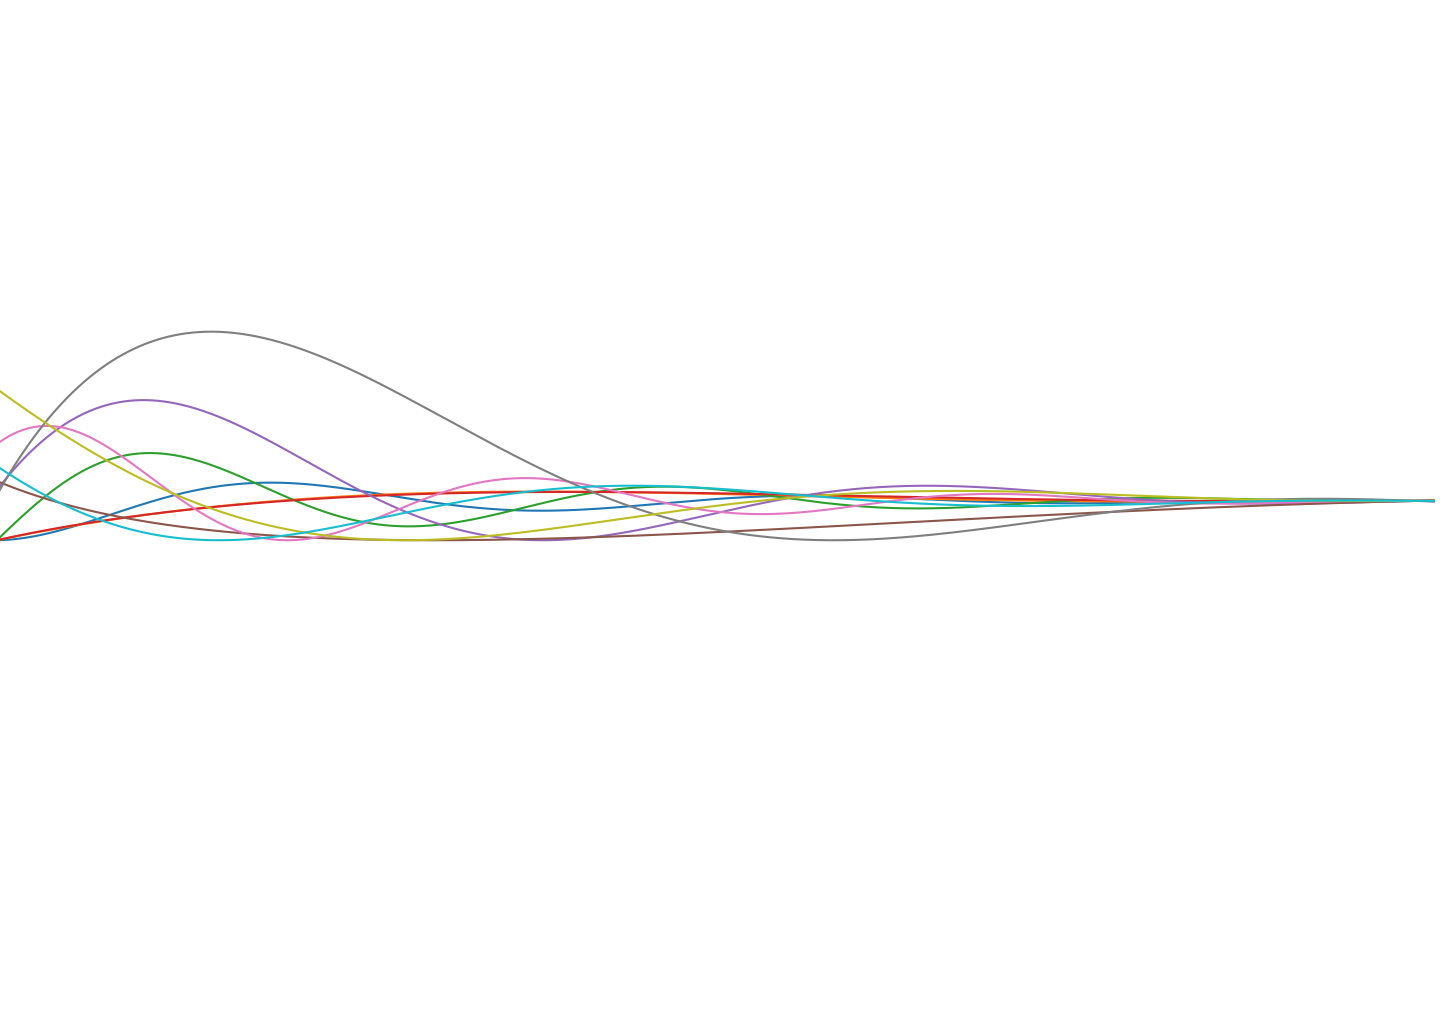
\includegraphics[width=\paperwidth,height=10cm]{header.png}};
    \MakeUppercase{\chaptertitlename}%
        \rlap{ \resizebox{!}{1.5cm}{\thechapter}}
  }
  {10pt}{\Huge}
\titlespacing*{\chapter}{0pt}{-30pt}{-5pt}

%Griffiths' style calligraphy font: use like $\scripty{r}$
\usepackage{calligra}
\DeclareMathAlphabet{\mathcalligra}{T1}{calligra}{m}{n}
\DeclareFontShape{T1}{calligra}{m}{n}{<->s*[2.2]callig15}{}
\newcommand{\scripty}[1]{\ensuremath{\mathcalligra{#1}}}

\begin{document}

\ctikzset{bipoles/length=.6cm}
\newcommand\esymbol[1]{\begin{circuitikz}
\draw (0,0) to [#1] (1,0); \end{circuitikz}}

\begin{titlepage}
	\centering
	{\scshape\LARGE Machine Learning \par}
	\vspace{1cm}
	{\huge\bfseries Condensed Notes \par}
	\vspace{1.5cm}
	{\scshape\Large \par}
	\vspace{2cm}
	{\Large\itshape Gabriel Sigurd Cabrera\par}
	\vfill
	\textsc{stk-in}4300 \& \textsc{fys-stk}4155	\vfill

% Bottom of the page
	{\large \today\par}
\end{titlepage}

\tableofcontents

\chapter{Introduction}

Given a set of features $\left\lbrace \mathbf{X}_1, \mathbf{X}_2, ..., \mathbf{X}_p \right\rbrace$ we can construct a \textit{learner}\label{vocab:learner0} that will use an outcome $\mathbf{Y}$ in order to predict other potential outcomes. This is called supervised learning.

There are several types of outcomes, \textbf{quantitative}\label{vocab:quantitative0}, \textbf{categorical}\label{vocab:categorical0}, and \textbf{ordered categorical} outcomes. The predicting task for a quantitative response is called \textbf{regression}\label{vocab:regression0}, and for a categorical response it is called \textbf{classification}\label{vocab:classification0}.

\textit{Quantitative} outcomes are binary\footnote{Meaning that they can be either \textit{True}, or \textit{False}} in nature, while \textit{categorical} outcomes can represent continuous or discrete non-binary values; \textit{ordered categorical} outcomes are a subcategory of categorical outcomes in which the outcomes are interrelated on a scale\footnote{This could be \textit{small}, \textit{medium}, and \textit{large}.}.

It is common to have three datasets - a \textbf{training set}\footnote{Used to train the algorithm to generate outputs in a specific way}\label{vocab:trainingset0}, a \textbf{test set}\footnote{Hidden dataset, to which the learner is not exposed.}\label{vocab:testset0} and a \textbf{validation set}\footnote{Optional in some cases, used to validate previous results with a third hidden dataset.}\label{vocab:validationset0}.

\section{Two Prediction Methods}

\subsection{Generalized Linear Models and Least Squares}

To predict a set of outputs $\hat{\mathbf{y}}$ based on a test input $\mathbf{X}$ we use the following model:

\begin{equation*}
\hat{\mathbf{y}} = \hat{\mathbf{X}}^\textsc{t} \hat{\beta}
\end{equation*}

Where $\mathbf{y}$ is an $(N \times O)$ matrix, $\mathbf{X}$ is an $(N \times p)$ matrix, and $\hat{\beta}$ is a $(p \times O)$ matrix, whose first row/element $\beta_0$ is called the \textbf{intercept}\label{vocab:intercept0} or \textbf{bias}\label{vocab:bias0}.  $\hat{\beta}$ itself is known as the \textbf{vector of coefficients}\label{vocab:vectorofcoefficients0}. This can also be visualized as follows:

\begin{equation*}
\begin{bmatrix}
\hat{y}_{1,1} & \hat{y}_{1,2} & \cdots & \hat{y}_{1,\textsc{o}} \\
\hat{y}_{2,1} & \hat{y}_{2,2} & \cdots & \hat{y}_{2,\textsc{o}} \\
\vdots & \vdots & \ddots & \vdots \\
\hat{y}_{\textsc{n},1} & \hat{y}_{\textsc{n},2} & \cdots & \hat{y}_{\textsc{n},\textsc{o}}
\end{bmatrix}
=
\begin{bmatrix}
X_{1,1} & X_{1,2} & \cdots & X_{1,p} \\
X_{2,1} & X_{2,2} & \cdots & X_{2,p} \\
\vdots & \vdots & \ddots & \vdots \\
X_{\textsc{n},1} & X_{\textsc{n},2} & \cdots & X_{\textsc{n},p}
\end{bmatrix}^\textsc{t}
\begin{bmatrix}
\hat{\beta}_{1,1} & \hat{\beta}_{1,2} & \cdots & \hat{\beta}_{1,\textsc{o}} \\
\hat{\beta}_{1,1} & \hat{\beta}_{1,2} & \cdots & \hat{\beta}_{1,\textsc{o}} \\
\vdots & \vdots & \ddots & \vdots \\
\hat{\beta}_{\textsc{n},1} & \hat{\beta}_{\textsc{n},2} & \cdots & \hat{\beta}_{\textsc{n},\textsc{o}}
\end{bmatrix}
\end{equation*}

Where each \textit{column} of the matrix $\mathbf{X}$ represents a \textbf{feature}\label{vocab:feature0} of the dataset, and each \textit{column} represents a single datapoint corresponding to an output in $\mathbf{y}$.

To find the vector of coefficients $\hat{\beta}$ we need a $(p \times N)$ set of inputs\footnote{Keep in mind that $\mathbf{X}^\textsc{t} \mathbf{X}$ must be \textit{nonsingular}!} $\mathbf{X}$ and their known outputs $\mathbf{y}$:

\begin{equation}
\label{eq_0}
\hat{\beta} = ( \mathbf{X}^\textsc{t} \mathbf{X} )^{-1} \mathbf{X}^\textsc{t} \mathbf{y}
\end{equation}

\begin{boxquote}
\textbf{Derivation of $\hat{\beta}$}

To find an expression for the vector of coefficients, it is necessary to minimize the distance between each point in a given dataset, and a predicted line.  This means we want to minimize something known as the \textbf{residual sum of squares}\label{vocab:RSS0}:

\begin{equation}
\label{eq_1}
\text{RSS}(\beta) = \sum_{i=1}^{N} (y_i - x_i^\textsc{t} \beta )^2
\end{equation}

Recall that functions can be minimized via differentiation.  We should rewrite equation \ref{eq_1} in vector form to accomplish this:

\begin{equation*}
\text{RSS} (\beta) = (\mathbf{y} - \mathbf{X}\beta)^\textsc{t} (\mathbf{y} - \mathbf{X}\beta)
\end{equation*}

We then take the derivative with respect to the vector of coefficients and set this to zero, keeping in mind that we must redefine some variable in the equation to take this into account.  We choose to put a hat on $\beta$:

\begin{equation*}
0 = \mathbf{X}^\textsc{t} (\mathbf{y} - \mathbf{X} \hat{\beta} )
\end{equation*}

Solving for $\hat{\beta}$ is the final step:

\begin{equation*}
\hat{\beta} = (\mathbf{X}^\textsc{t} \mathbf{X})^{-1} \mathbf{X}^\textsc{t} \mathbf{y}
\end{equation*}

\end{boxquote}

\subsubsection{Quick Notation Reference}

\begin{table}[H]
\caption{Dimensions Guide\label{table_0}}
\centering
\begin{tabular}{| c l|}
\hline
\textbf{Symbol} & \textbf{Description} \\
\hline
$N$ & Number of datapoints \\
$p$ & Number of dimensions/attributes \\
$O$ & Number of outputs per datapoint \\
\hline
\end{tabular}
\end{table}

\begin{table}[H]
\caption{Notation Guide\label{table_1}}
\centering
\begin{tabular}{| c l c |}
\hline
\textbf{Symbol} & \textbf{Description} & \textbf{Dimensions} \\
\hline
$\mathbf{X}$ & Input matrix & $N \times p$ \\
$x_i$ & Column vector of a row in $\mathbf{X}$ & $p \times 1$ \\
$\mathbf{X}_j$ & Column vector of a column in $\mathbf{X}$ & $N \times 1$ \\
$\mathbf{y}$ & Expected output matrix & $N \times O$ \\
$y_i$ & Row vector of a row in $\mathbf{y}$ & $1 \times O$ \\
$\hat{Y}$ & Predicted output matrix & $N \times O$ \\
\hline
\end{tabular}
\end{table}

\subsection{Nearest-Neighbor Methods}



\chapter{Glossary}

\begin{table}[H]
\caption{Useful terms, where they appear in the text, and potential synonyms\label{table_2}}
\centering
\begin{tabular}{| l l l |}
\hline
\textbf{Term} & \textbf{Page} & \textbf{Synonyms} \\
\hline
Bias & \pageref{vocab:bias0} & Intercept \\
Categorical & \pageref{vocab:categorical0} & Discrete, Qualitative \\
Cost Function & TEMPORARY & Error Function, Loss Function \\
Classification & \pageref{vocab:classification0} & N/A \\
Discrete & \pageref{vocab:categorical0} & Categorical, Qualitative \\
Error Function & TEMPORARY & Cost Function, Loss Function \\
Feature & \pageref{vocab:feature0} & N/A \\
Intercept & \pageref{vocab:intercept0} & Bias \\
Learner & \pageref{vocab:learner0} & N/A \\
Loss Function & TEMPORARY & Cost Function, Error Function \\
Qualitative & \pageref{vocab:categorical0} & Categorical, Discrete \\
Quantitative & \pageref{vocab:quantitative0} & N/A \\
Regression & \pageref{vocab:regression0} & N/A \\
Residual Sum of Squares & \pageref{vocab:RSS0} & N/A \\
Test Set & \pageref{vocab:testset0} & N/A \\
Training Set & \pageref{vocab:trainingset0} & N/A \\
Validation Set & \pageref{vocab:validationset0} & N/A \\
Vector of Coefficients & \pageref{vocab:vectorofcoefficients0} & N/A \\
\hline
\end{tabular}
\end{table}

\bibliography{bib}{}
\bibliographystyle{IEEEtran}

\end{document}
